\documentclass{article}
\usepackage{tikz}
\usetikzlibrary{automata,arrows.meta}

\begin{document}

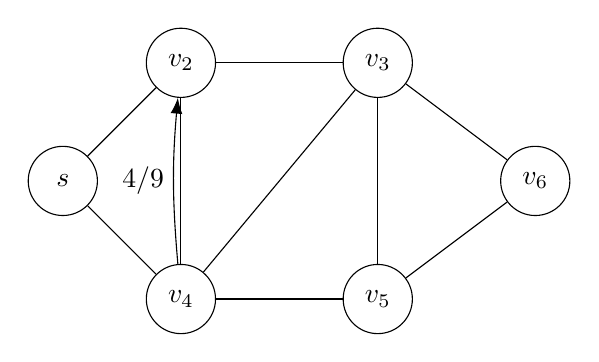
\begin{tikzpicture}


    \node[draw,circle,minimum size=25] (v1)  at (-5,1.5) {$s$};
    \node[draw,circle,minimum size=25] (v2) at (-3.5,3) {$v_2$};
    \node[draw,circle,minimum size=25] (v4) at (-3.5,0) {$v_4$};
    \node[draw,circle,minimum size=25] (v3) at (-1,3) {$v_3$};
    \node[draw,circle,minimum size=25] (v5) at (-1,0) {$v_5$};
    \node[draw,circle,minimum size=25] (v6) at (1,1.5) {$v_6$};
    \draw  (v1) edge (v2);
    \draw  (v2) edge (v3);
    \draw  (v1) edge (v4);
    \draw[-{Latex[length=2mm]}]  (v4) edge [bend left=5] node[midway,left]{4/9} (v2);
    \draw  (v4) edge (v5);
    \draw  (v3) edge (v5);
    \draw  (v5) edge (v6);
    \draw  (v3) edge (v6);
    \draw  (v4) edge (v3);
    \draw  (v3) edge (v2);
    \draw  (v2) edge (v4);
    \end{tikzpicture}
    \end{document}
